\documentclass[10pt,twocolumn]{article}

\usepackage[margin=0.75in]{geometry}
\usepackage[T1]{fontenc}
\usepackage[utf8]{inputenc}
\usepackage{times}
\usepackage{microtype}
\usepackage{graphicx}
\usepackage{booktabs}
\usepackage{amsmath}
\usepackage{array}
\usepackage{multirow}
\usepackage{xcolor}
\usepackage{hyperref}
\usepackage{caption}

\hypersetup{
  colorlinks=true,
  linkcolor=blue,
  citecolor=blue,
  urlcolor=blue
}

\graphicspath{{poster_figures/}}
\setlength{\textfloatsep}{8pt plus 1pt minus 2pt}
\setlength{\floatsep}{8pt plus 1pt minus 2pt}
\setlength{\intextsep}{8pt plus 1pt minus 2pt}

\title{\textbf{Reducing Hallucination in LLaVA-1.5-7B via Causally Targeted LoRA and Inference-Time Attention Grounding}}
\author{
Armaan Sandhu \and
Hima Jagadeesha Kammachi \and
Abhilasha Senapati
\\
\small University of Massachusetts Amherst
\\
\small \texttt{apsandhu@umass.edu}
\quad
\small \texttt{hkammachi@umass.edu}
\quad
\small \texttt{asenapati@umass.edu}
}
\date{}

\begin{document}
\maketitle

\begin{abstract}
Vision-language models such as LLaVA-1.5-7B often hallucinate objects that are not present in the image, especially during open-ended caption generation. In this project, we revisit our proposal that hallucination may be concentrated in a small set of attention heads and can therefore be reduced through targeted intervention rather than full-model adaptation. We implement a mixed mitigation strategy with three components: (1) causal and screening-based identification of hallucination-linked heads, (2) surgical LoRA fine-tuning restricted to those heads, and (3) an inference-time attention-grounding controller that suppresses object-word logits when visual grounding becomes weak. Our final system updates 32 of 1024 attention heads, or about 3.1\% of the model's attention space. On a 400-image COCO evaluation, the combined method reduces caption-level hallucination rate from 0.370 to 0.230 and object-level hallucination rate from 0.156 to 0.096. At the same time, the gains come with shorter captions and a small drop in ground-truth object recall. Overall, the final results support the main hypothesis of the proposal: targeted intervention on a small set of heads can meaningfully reduce hallucination, but strong hallucination suppression must be balanced against fluency and content coverage.
\end{abstract}

\section{Introduction}
Large vision-language models frequently produce fluent but visually unsupported statements. In LLaVA-1.5-7B, this issue appears as object hallucination: the model names entities that are absent from the image or over-commits to plausible scene details without enough visual support. This behavior reduces reliability in downstream settings where factual grounding matters more than stylistic fluency.

Our original proposal was built around a specific interpretability hypothesis: hallucination may be partially concentrated in a small set of attention heads and can therefore be reduced by editing those heads directly. The final project keeps that framing and develops it into a complete mitigation pipeline for LLaVA-1.5-7B~\cite{liu2024llava}. Rather than relying on a single intervention, we combine targeted model adaptation with a lightweight decoding controller.

We pursue three concrete objectives:
\begin{enumerate}
  \item Identify hallucination-prone heads using screening and causal validation.
  \item Reduce hallucination through head-targeted LoRA rather than broad full-model adaptation.
  \item Add an inference-time grounding mechanism that discourages object mentions when visual attention becomes weak.
\end{enumerate}

The final results support the central idea while also exposing an important tradeoff. Updating only 32 out of 1024 attention heads reduces hallucination substantially, and grounding-aware decoding improves the adapted model further. However, stronger suppression also shortens captions and slightly lowers object recall. We therefore present the report not as a claim that hallucination is solved, but as evidence that targeted intervention is both effective and limited in predictable ways.

\section{Related work}
Our project draws from three main directions. First, LLaVA-style instruction-tuned vision-language models achieve strong multimodal generation quality, but they also inherit familiar language-model tendencies toward overconfident completion and visually unsupported detail~\cite{liu2024llava}. Second, prior work on image-caption hallucination formalized this issue through metrics such as CHAIR, which measures whether generated captions include objects absent from the image annotations~\cite{rohrbach2018object}. Third, parameter-efficient adaptation methods such as LoRA and QLoRA show that important model behaviors can often be changed through small low-rank updates rather than expensive full fine-tuning~\cite{hu2022lora,dettmers2024qlora}.

We also build on the preference-learning perspective behind DPO~\cite{rafailov2024dpo}. In our setting, the contrast is between a grounded reference caption and the model's own hallucinated alternative, allowing us to push the model toward more visually supported language without introducing a separate reward model.

The main difference between our approach and a standard LoRA pipeline is that we do not treat all attention heads as equally important. We first use causal evidence to localize a shortlist of heads associated with hallucination, then confine adaptation to those heads, and finally add a decoding-time residual safety mechanism based on attention grounding.

\section{Technical approach}
\subsection{Model and setup}
Our base model is \texttt{llava-hf/llava-1.5-7b-hf}. Stage 1 and the inference-time controller require access to attention tensors, so those stages run in fp16 with eager attention. Stage 2 uses a QLoRA-style setup because it only needs logits rather than attention weights. All stages use COCO val2014 images and annotations~\cite{lin2014coco}.

\subsection{Stage 1: Causal head identification}
We begin with a screening pass over 200 COCO validation images. For each generated caption, we record per-head attention during noun generation and score all 1024 attention heads by how much their visual attention decreases when the model emits a hallucinated object word rather than a grounded one. This gives a fast first-pass ranking of candidate heads.

We then validate the strongest candidates causally. The top-ranked heads are ablated one at a time by zeroing their contribution and measuring the change in hallucination-token log-probability. This stage narrows the search to 32 heads across 19 transformer layers. These heads form the shared target set for both fine-tuning and inference-time control.

\begin{figure*}[t]
  \centering
  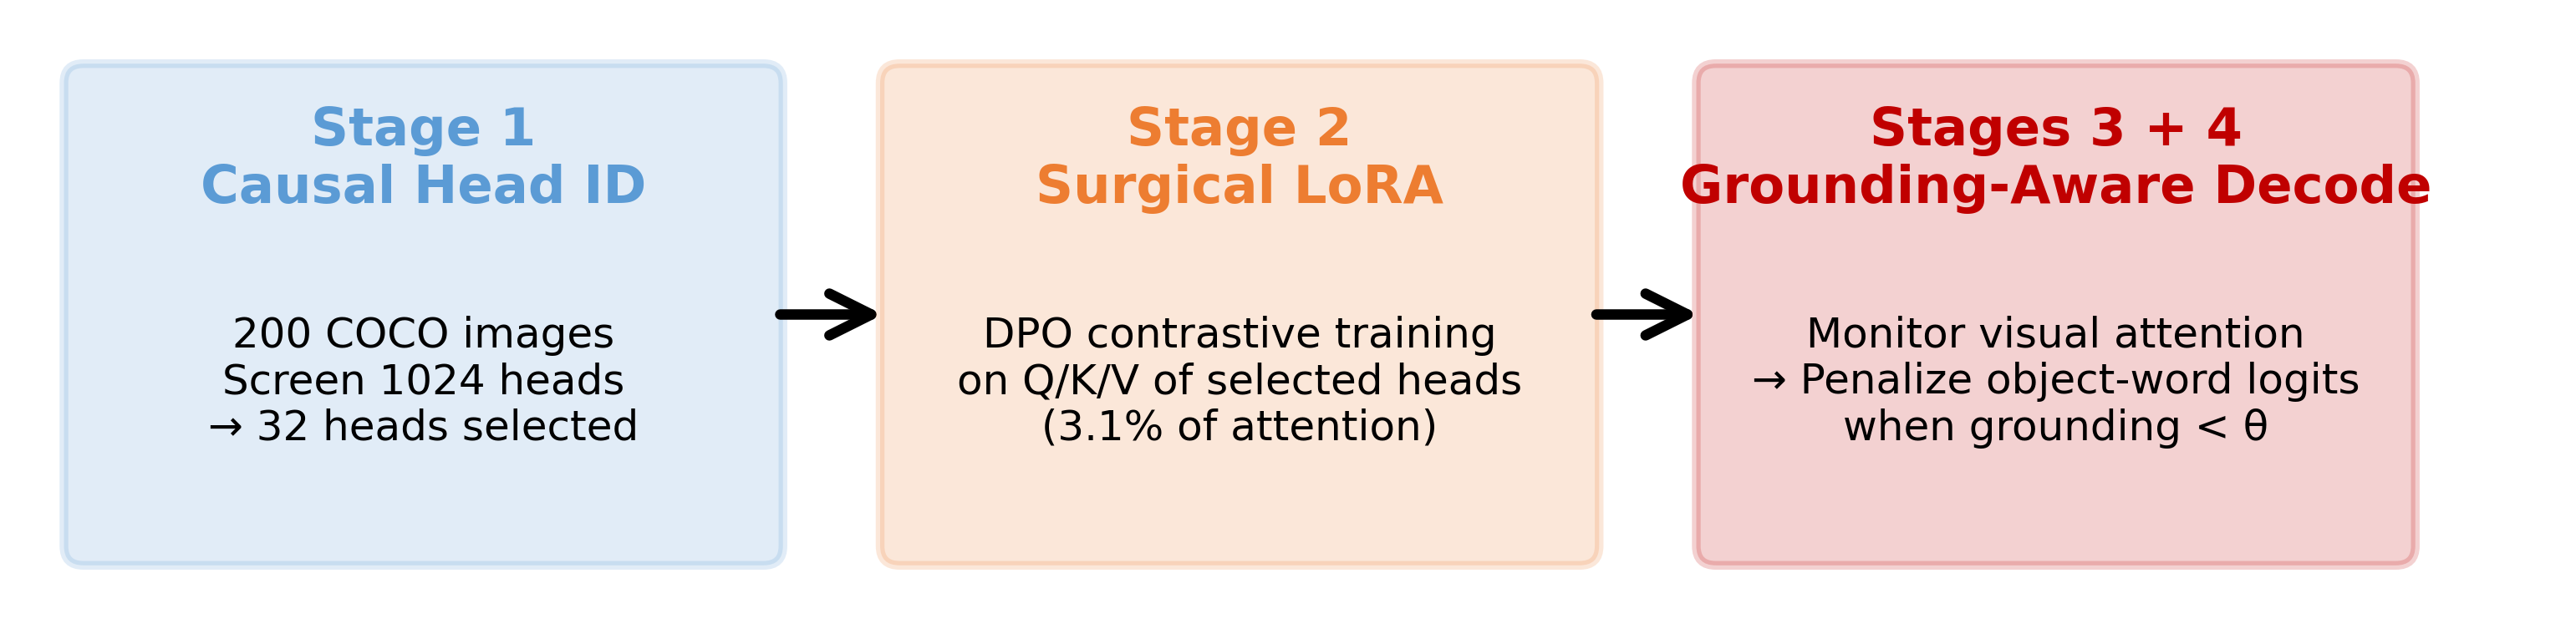
\includegraphics[width=0.95\textwidth]{diagram1_pipeline.png}
  \caption{Overall project pipeline. We first identify hallucination-linked heads, then train a surgical LoRA adapter on those heads, and finally add grounding-aware decoding.}
  \label{fig:pipeline}
\end{figure*}

\subsection{Stage 2: Surgical LoRA}
Stage 2 applies QLoRA-style fine-tuning, but only within the layers that contain the identified heads. LoRA is attached to the Q/K/V projections of those layers, and gradient masking further restricts updates to the exact head slices of interest. In effect, only 32 of 1024 attention heads are allowed to change, while the rest of the model remains frozen.

Training uses contrastive caption pairs derived from COCO. For each image, the chosen response is a ground-truth COCO caption and the rejected response is the model's own hallucinated caption obtained in Stage 1. We optimize a DPO-style objective with LoRA rank $r=8$, $\alpha=16$, dropout $0.05$, and three epochs. The goal is to move the selected heads toward grounded caption behavior without performing broad model adaptation.

\subsection{Stages 3 and 4: Inference-time attention grounding}
The third component is a training-free decoding controller. At each generation step, we compute a grounding score from the average visual attention mass assigned by the selected heads to image tokens. When this score falls below a threshold $\theta$, we penalize logits corresponding to likely object words from a COCO-derived vocabulary. Intuitively, when the selected heads appear weakly grounded, the decoder should become more conservative about naming objects.

Stage 3 evaluates this controller on the base model. Stage 4 applies the same controller on top of the LoRA-adapted model. The resulting combined system is our final method:
\[
g_t = \mathrm{mean}_{h \in H} \frac{\sum_{i \in \mathrm{img}} \alpha_{h,i}}{\sum_j \alpha_{h,j}},
\qquad
\ell_v \leftarrow \ell_v + \alpha (g_t - \theta)
\]
for object-word token $v$ when $g_t < \theta$. This controller is simple by design: it does not claim to prove grounding, but it provides an interpretable residual safeguard at inference time.

\section{Experimental setup}
We evaluate mainly with CHAIRs and CHAIRi~\cite{rohrbach2018object}. CHAIRs measures the fraction of captions that contain at least one hallucinated object mention, while CHAIRi measures the fraction of object mentions that are hallucinated. We also track average caption length and ground-truth object recall, since hallucination can be reduced in a trivial way if the model simply becomes shorter and less specific.

The final report focuses on the 400-image evaluation summarized in the poster, since that is the most complete end-of-project result. Earlier 40-image notebook experiments were useful for development and debugging, but they were too small and sometimes produced unstable caption behavior. We therefore use them as supporting evidence rather than the main claim.

Our final comparison uses four conditions:
\begin{itemize}
  \item \textbf{Baseline:} original LLaVA-1.5-7B.
  \item \textbf{LoRA only:} Stage 2 adapter, no grounding control.
  \item \textbf{Grounding only:} Stage 3 controller, no LoRA.
  \item \textbf{LoRA + Grounding:} full system.
\end{itemize}

\section{Results and analysis}
\subsection{Main quantitative results}
Table~\ref{tab:main-results} shows the final 400-image results reported in the poster. The combined system gives the best hallucination scores: CHAIRs improves from 0.370 to 0.230 and CHAIRi improves from 0.156 to 0.096. This corresponds to a 38\% relative reduction in caption-level hallucination and a 39\% relative reduction in object-level hallucination.

LoRA alone already provides a strong gain, reducing CHAIRs to 0.265 and CHAIRi to 0.104. Grounding alone gives a smaller but still meaningful improvement, suggesting that inference-time control helps but is not strong enough to replace model adaptation. The strongest performance appears when both mechanisms are combined.

\begin{table}[t]
  \centering
  \caption{Final evaluation on 400 images. Lower is better for CHAIR; higher is better for recall.}
  \label{tab:main-results}
  \small
  \begin{tabular}{lcccc}
    \toprule
    Method & CHAIRs & CHAIRi & Length & Recall \\
    \midrule
    Baseline & 0.370 & 0.156 & 61.1 & \textbf{0.78} \\
    LoRA only & 0.265 & 0.104 & 27.6 & 0.74 \\
    Grounding only & 0.310 & 0.141 & \textbf{62.1} & 0.74 \\
    LoRA + Grounding & \textbf{0.230} & \textbf{0.096} & 29.6 & 0.70 \\
    \bottomrule
  \end{tabular}
\end{table}

\begin{figure*}[t]
  \centering
  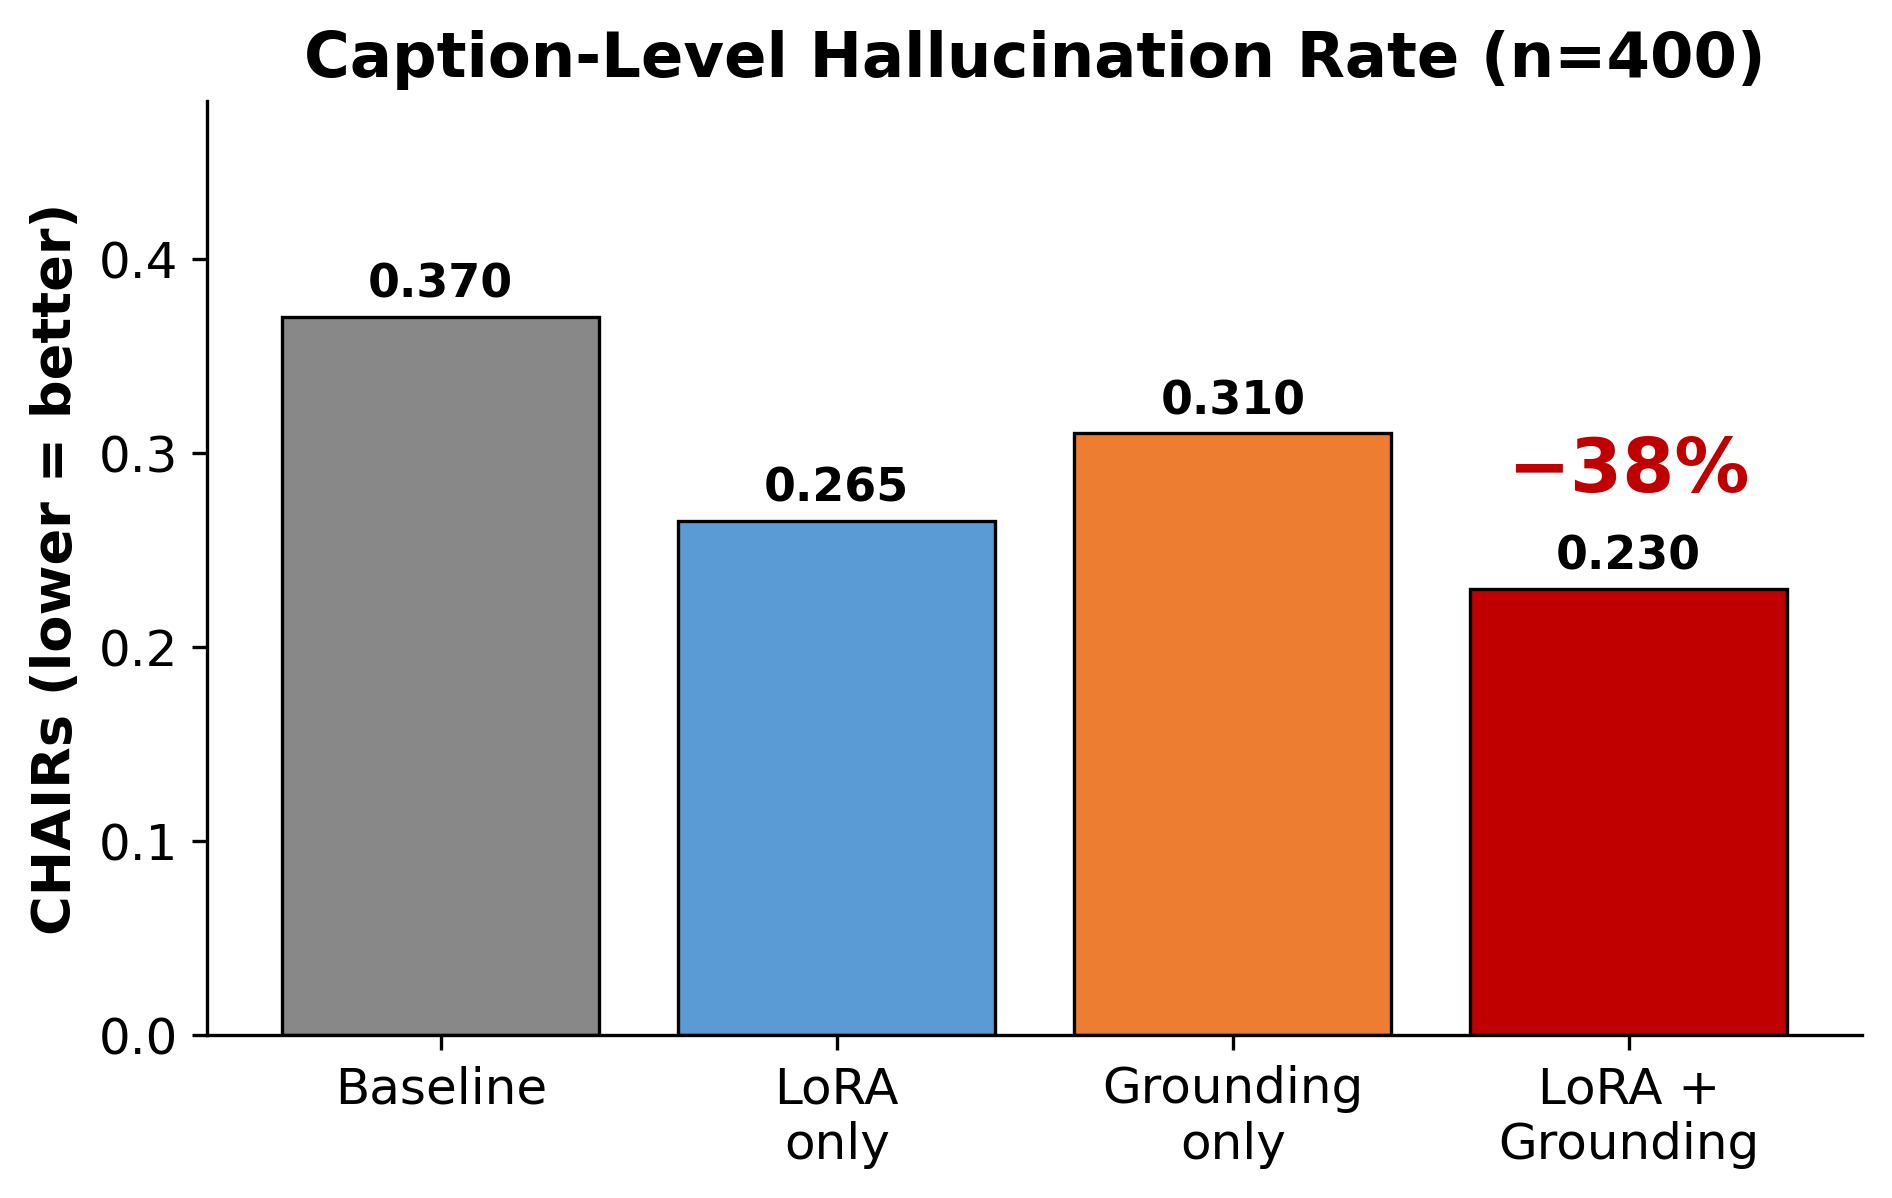
\includegraphics[width=0.47\textwidth]{fig1_chairs_bars.png}
  \hfill
  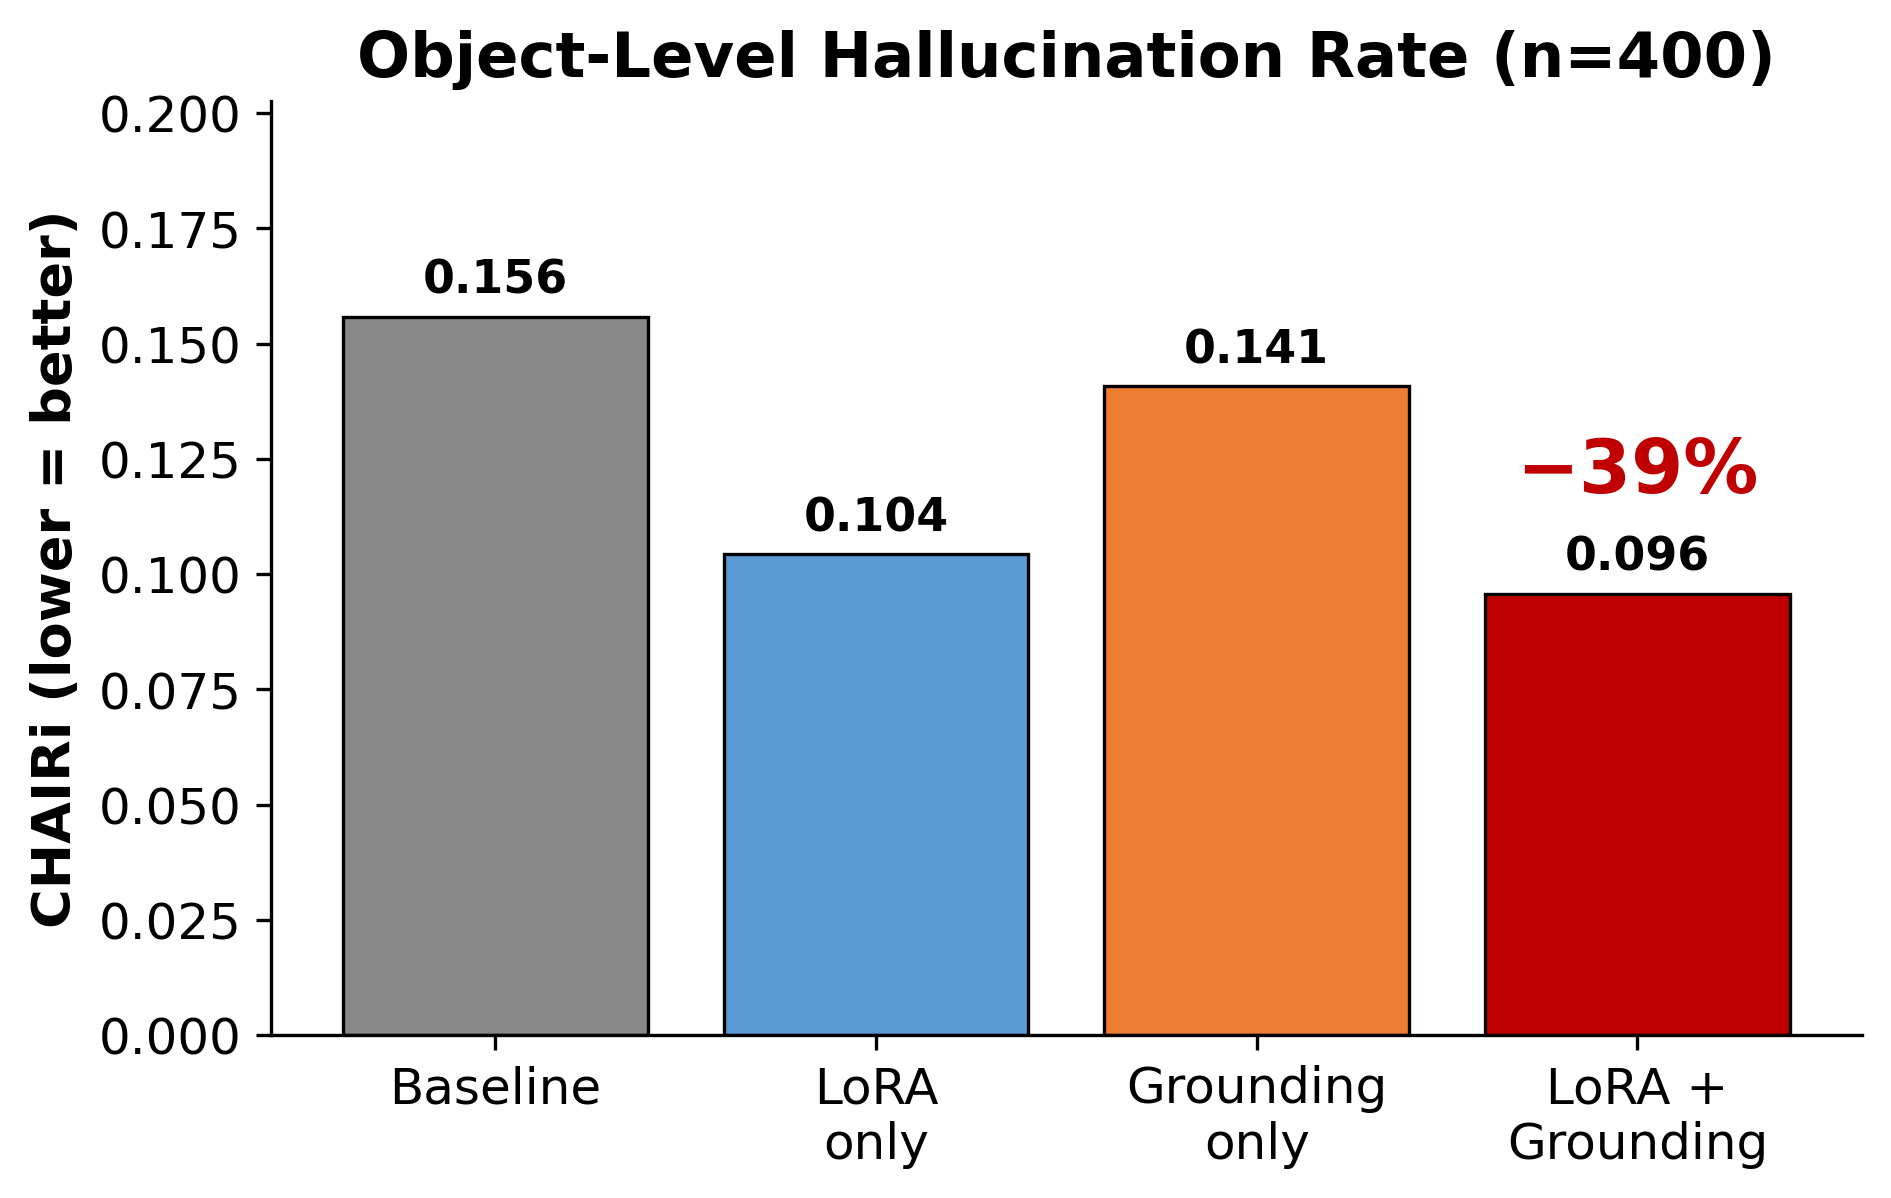
\includegraphics[width=0.47\textwidth]{fig2_chairi_bars.png}
  \caption{Final hallucination results on 400 images. The combined system gives the lowest caption-level and object-level hallucination rates.}
  \label{fig:main-bars}
\end{figure*}

\subsection{Grounding helps most when LoRA is already useful}
Figure~\ref{fig:lora-scale} clarifies the interaction between the two components. Across all tested LoRA scales in a 200-image sweep, adding grounding improves CHAIRs relative to LoRA alone. The gain is modest at weak LoRA scales and largest at full adapter strength, where the gap is 0.035. This matches the main 400-image result: grounding control adds value, but it is most effective after the model has already been shifted toward grounded behavior.

\begin{figure}[t]
  \centering
  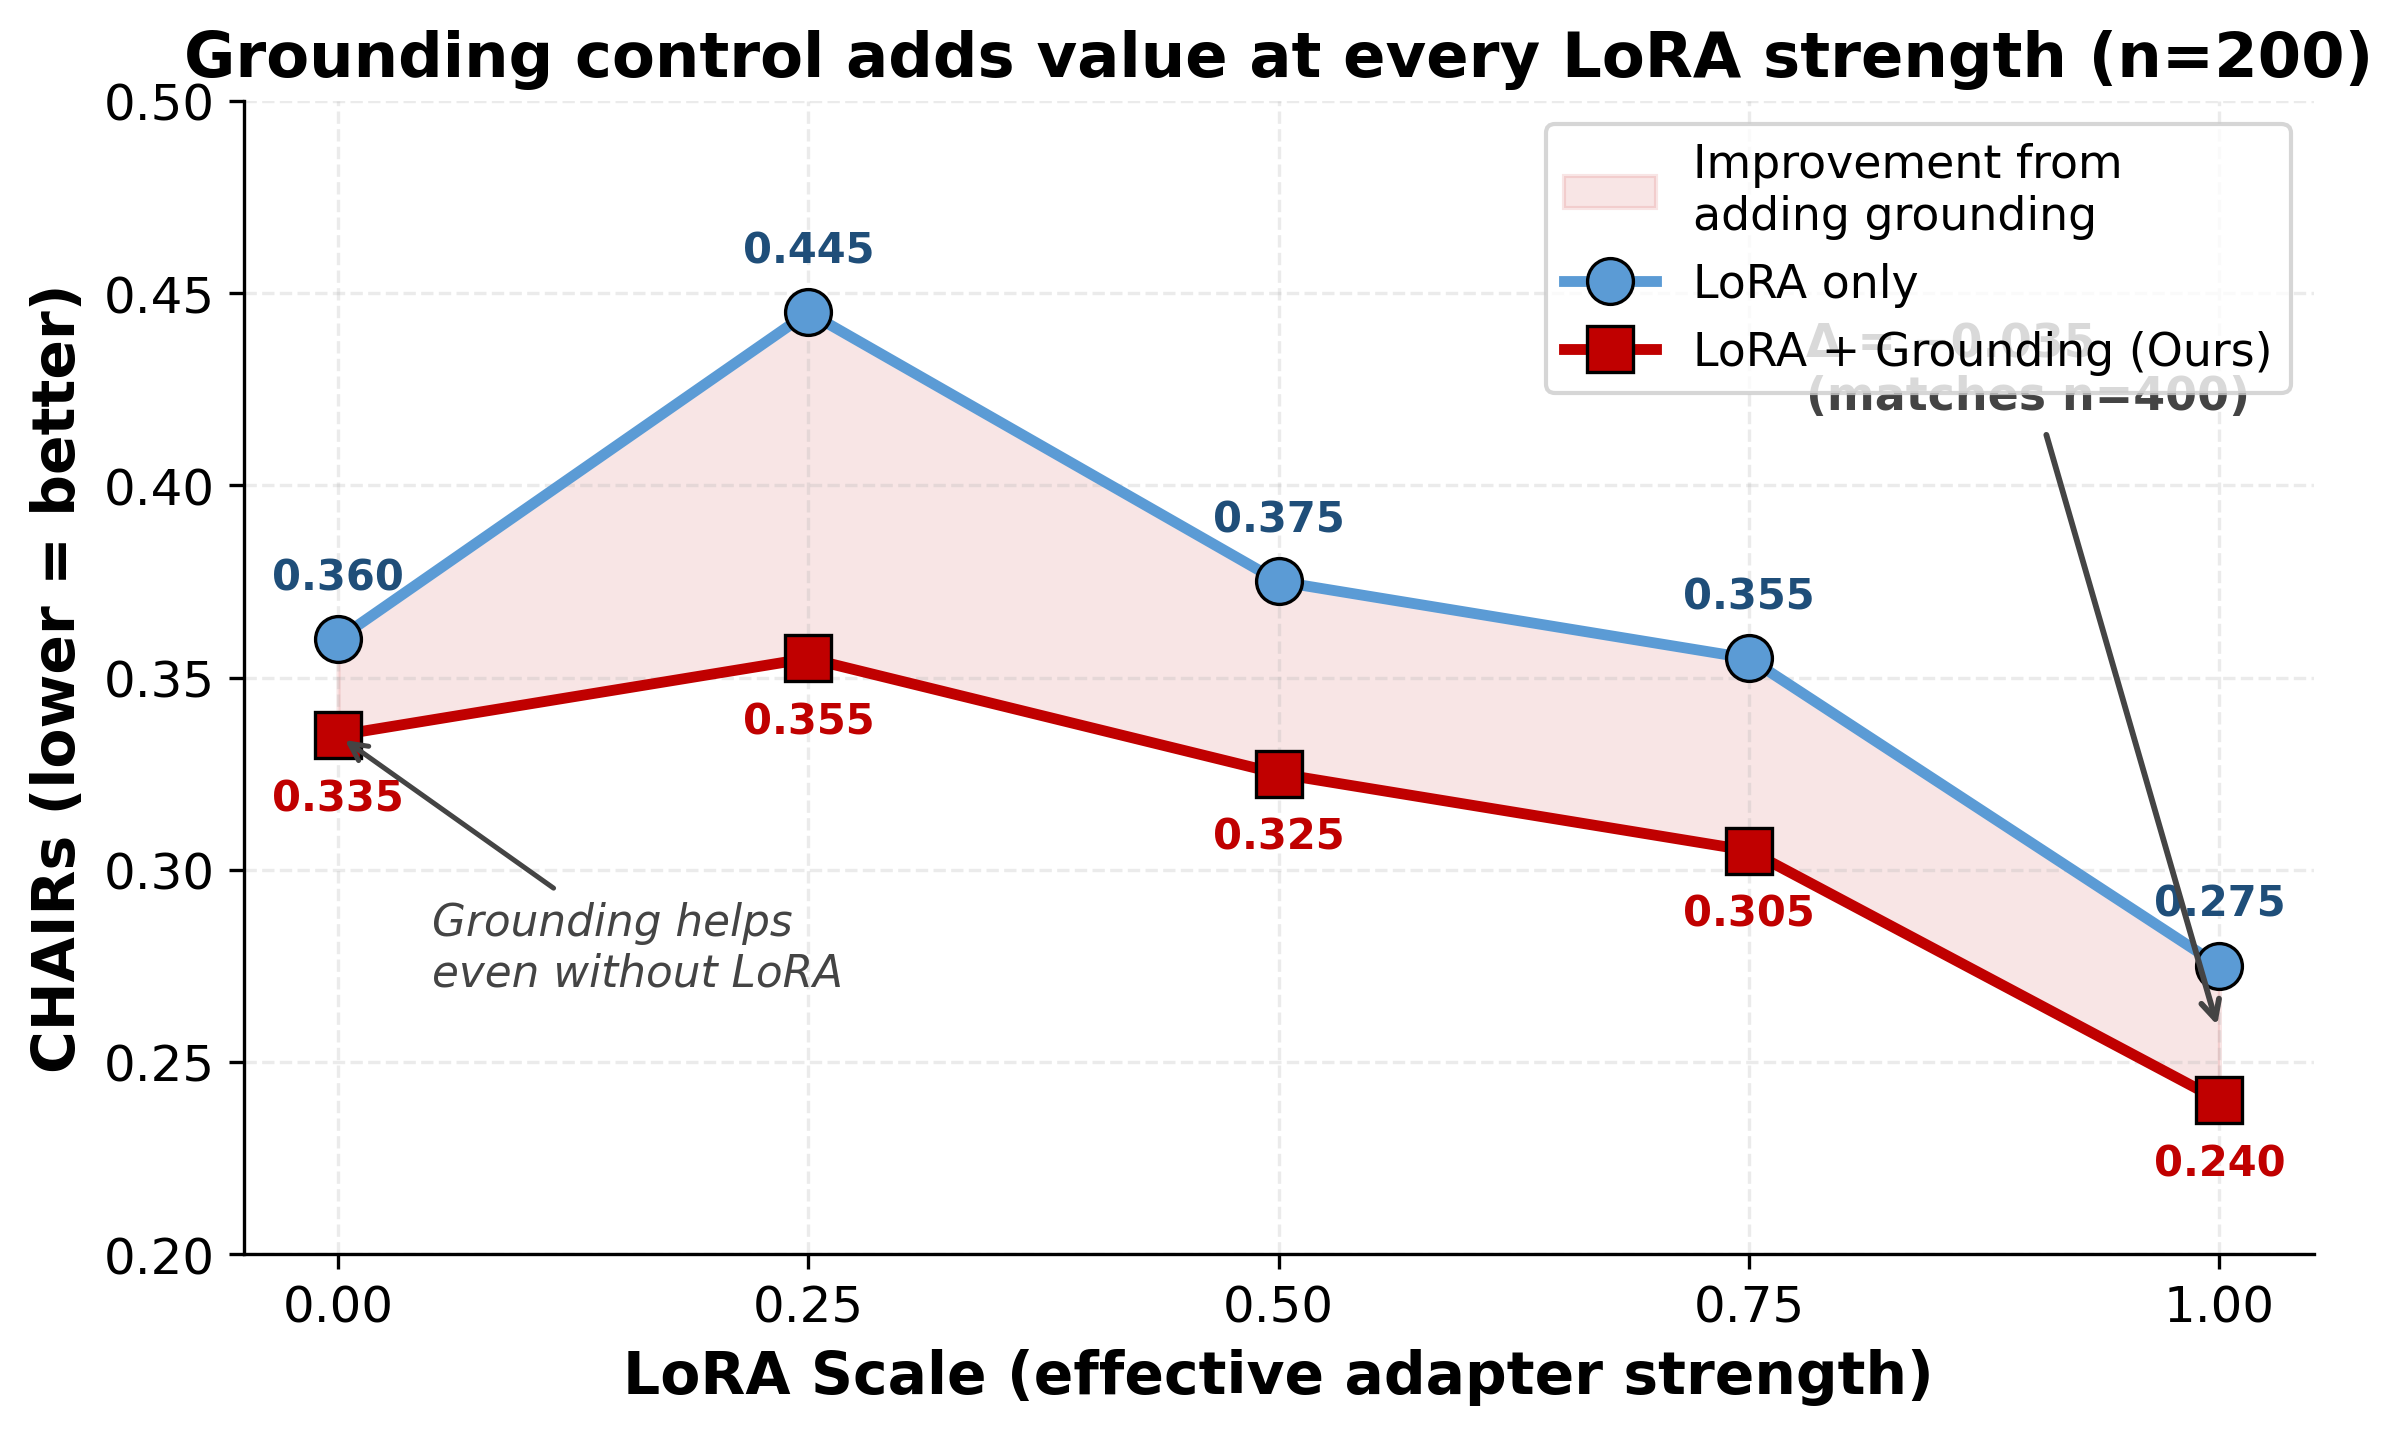
\includegraphics[width=\columnwidth]{fig_lora_scale_sweep.png}
  \caption{Grounding control consistently improves CHAIRs across LoRA strengths in the poster sweep.}
  \label{fig:lora-scale}
\end{figure}

\subsection{Threshold and head-count ablations}
We also tested sensitivity to the grounding threshold and the number of selected heads. The threshold sweep over $\theta \in \{0.04, 0.06, 0.08, 0.10, 0.12\}$ stays in a narrow band: CHAIRs ranges from 0.24 to 0.26 and CHAIRi stays near 0.10. This suggests that the controller is reasonably stable once the threshold is set within a plausible operating range.

The top-16 versus top-32 comparison is more mixed. In the poster ablation, both settings produce almost identical scores. This still supports the Stage 1 ranking, since a small subset of heads is clearly enough to carry most of the effect, but it also suggests that the final performance may be driven by the strongest part of the shortlist rather than the full set.

\subsection{Caption length and recall tradeoff}
The largest gains in hallucination are accompanied by a visible change in caption behavior. LoRA-only and LoRA+Grounding both produce much shorter captions than the baseline, while ground-truth object recall drops from 0.78 in the baseline to 0.70 in the final system. This makes the tradeoff concrete: the model becomes safer in terms of unsupported object mentions, but also more conservative in how much it says.

\begin{figure*}[t]
  \centering
  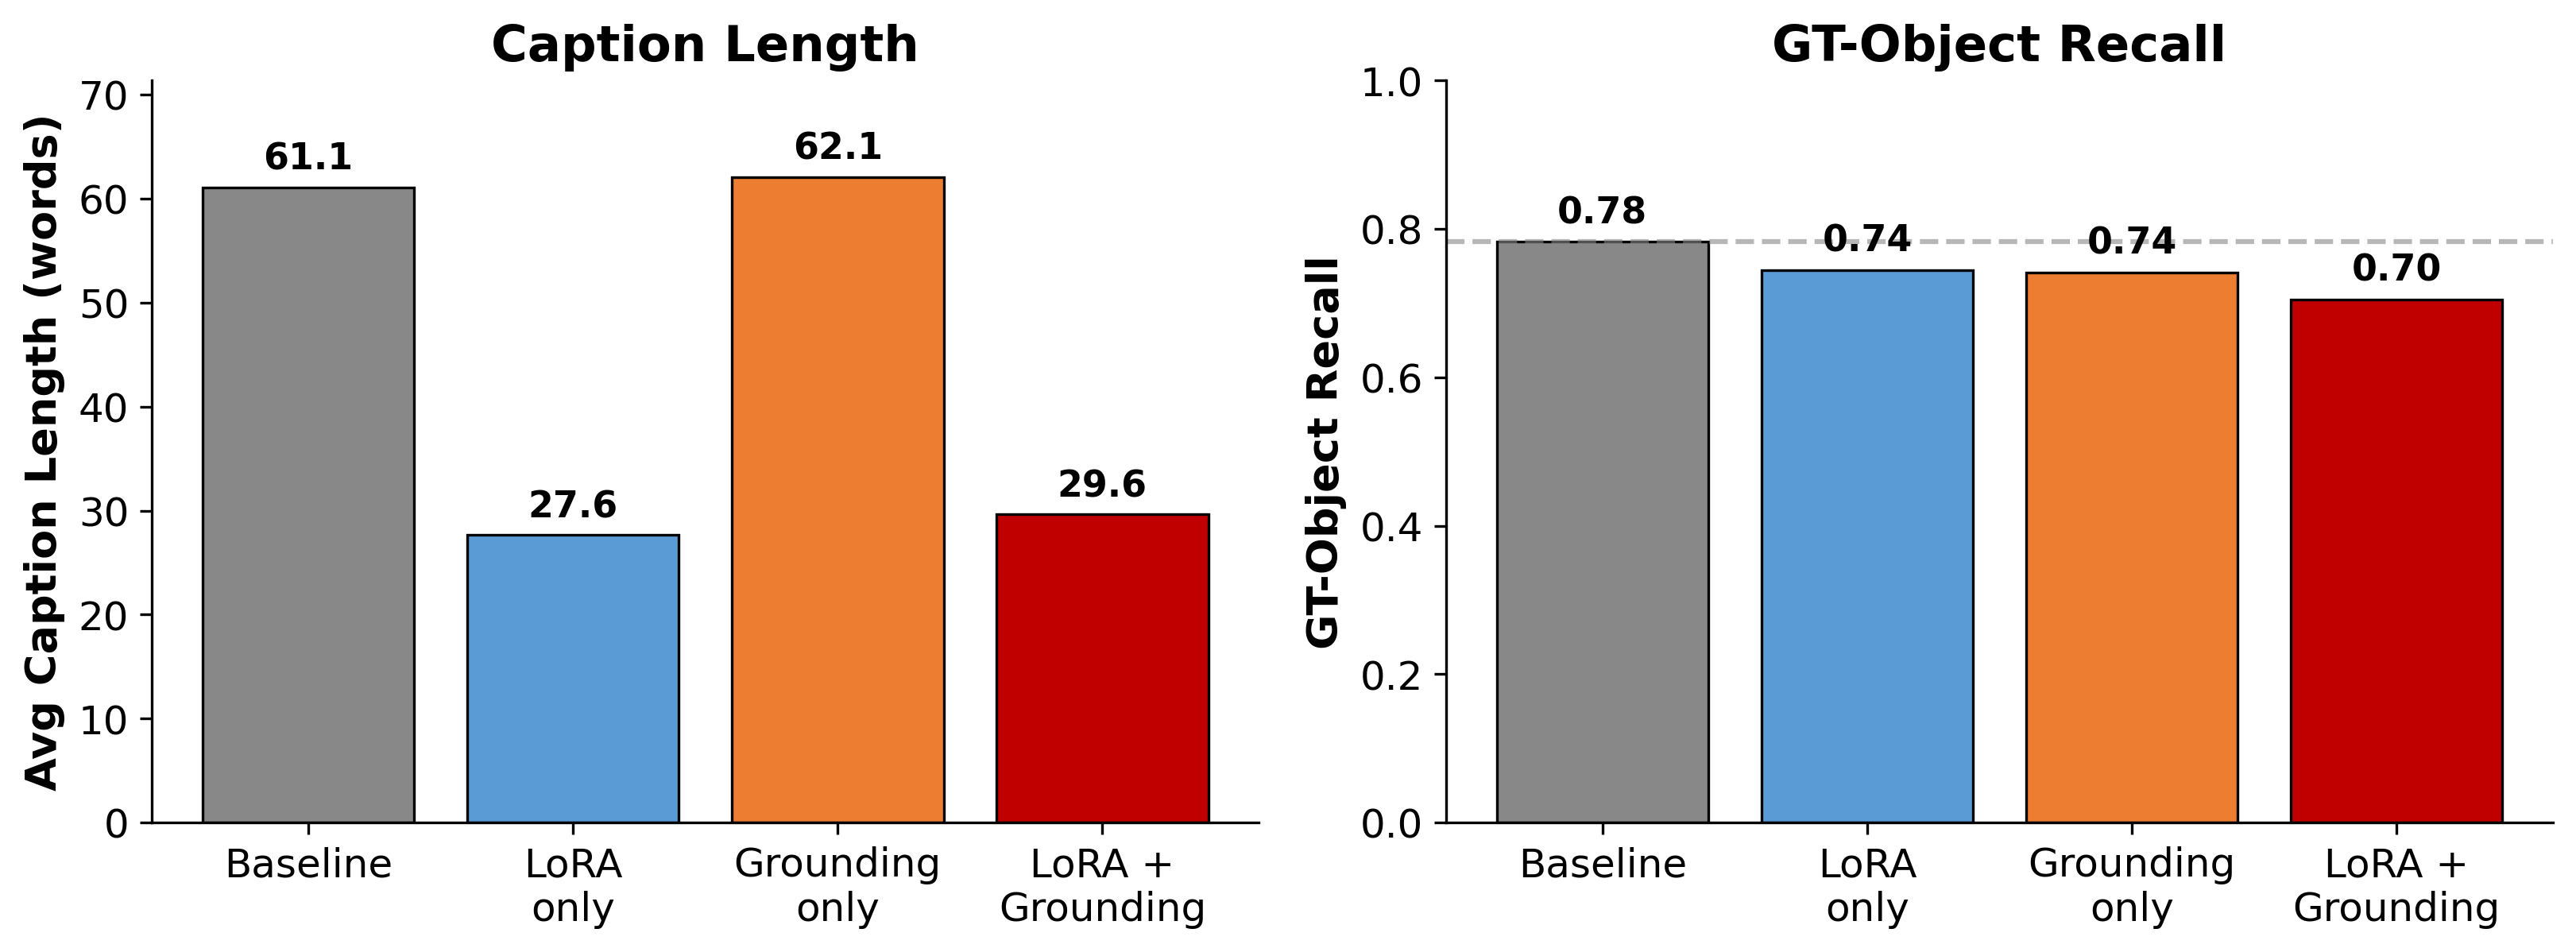
\includegraphics[width=0.95\textwidth]{fig3_length_recall.png}
  \caption{Auxiliary metrics from the poster. Hallucination reduction is accompanied by shorter captions and a modest drop in object recall.}
  \label{fig:length-recall}
\end{figure*}

\subsection{Qualitative behavior}
The qualitative examples reveal the same pattern. The combined method is often more cautious and makes fewer unsupported object claims, but it can also become terse. In Figure~\ref{fig:qualitative}, the baseline fails to mention the COCO objects, LoRA-only mentions the correct object but also hallucinates ``man,'' and the combined model preserves the correct object mention without adding the extra hallucinated object. This is representative of the kind of correction we hoped to obtain.

At the same time, some intermediate notebook outputs showed a harsher version of the same trend, where CHAIR improved but the caption quality degraded into short or repetitive text. This is one reason we report the more conservative poster-scale numbers as the main result and explicitly include caption length and recall in the analysis.

\begin{figure*}[t]
  \centering
  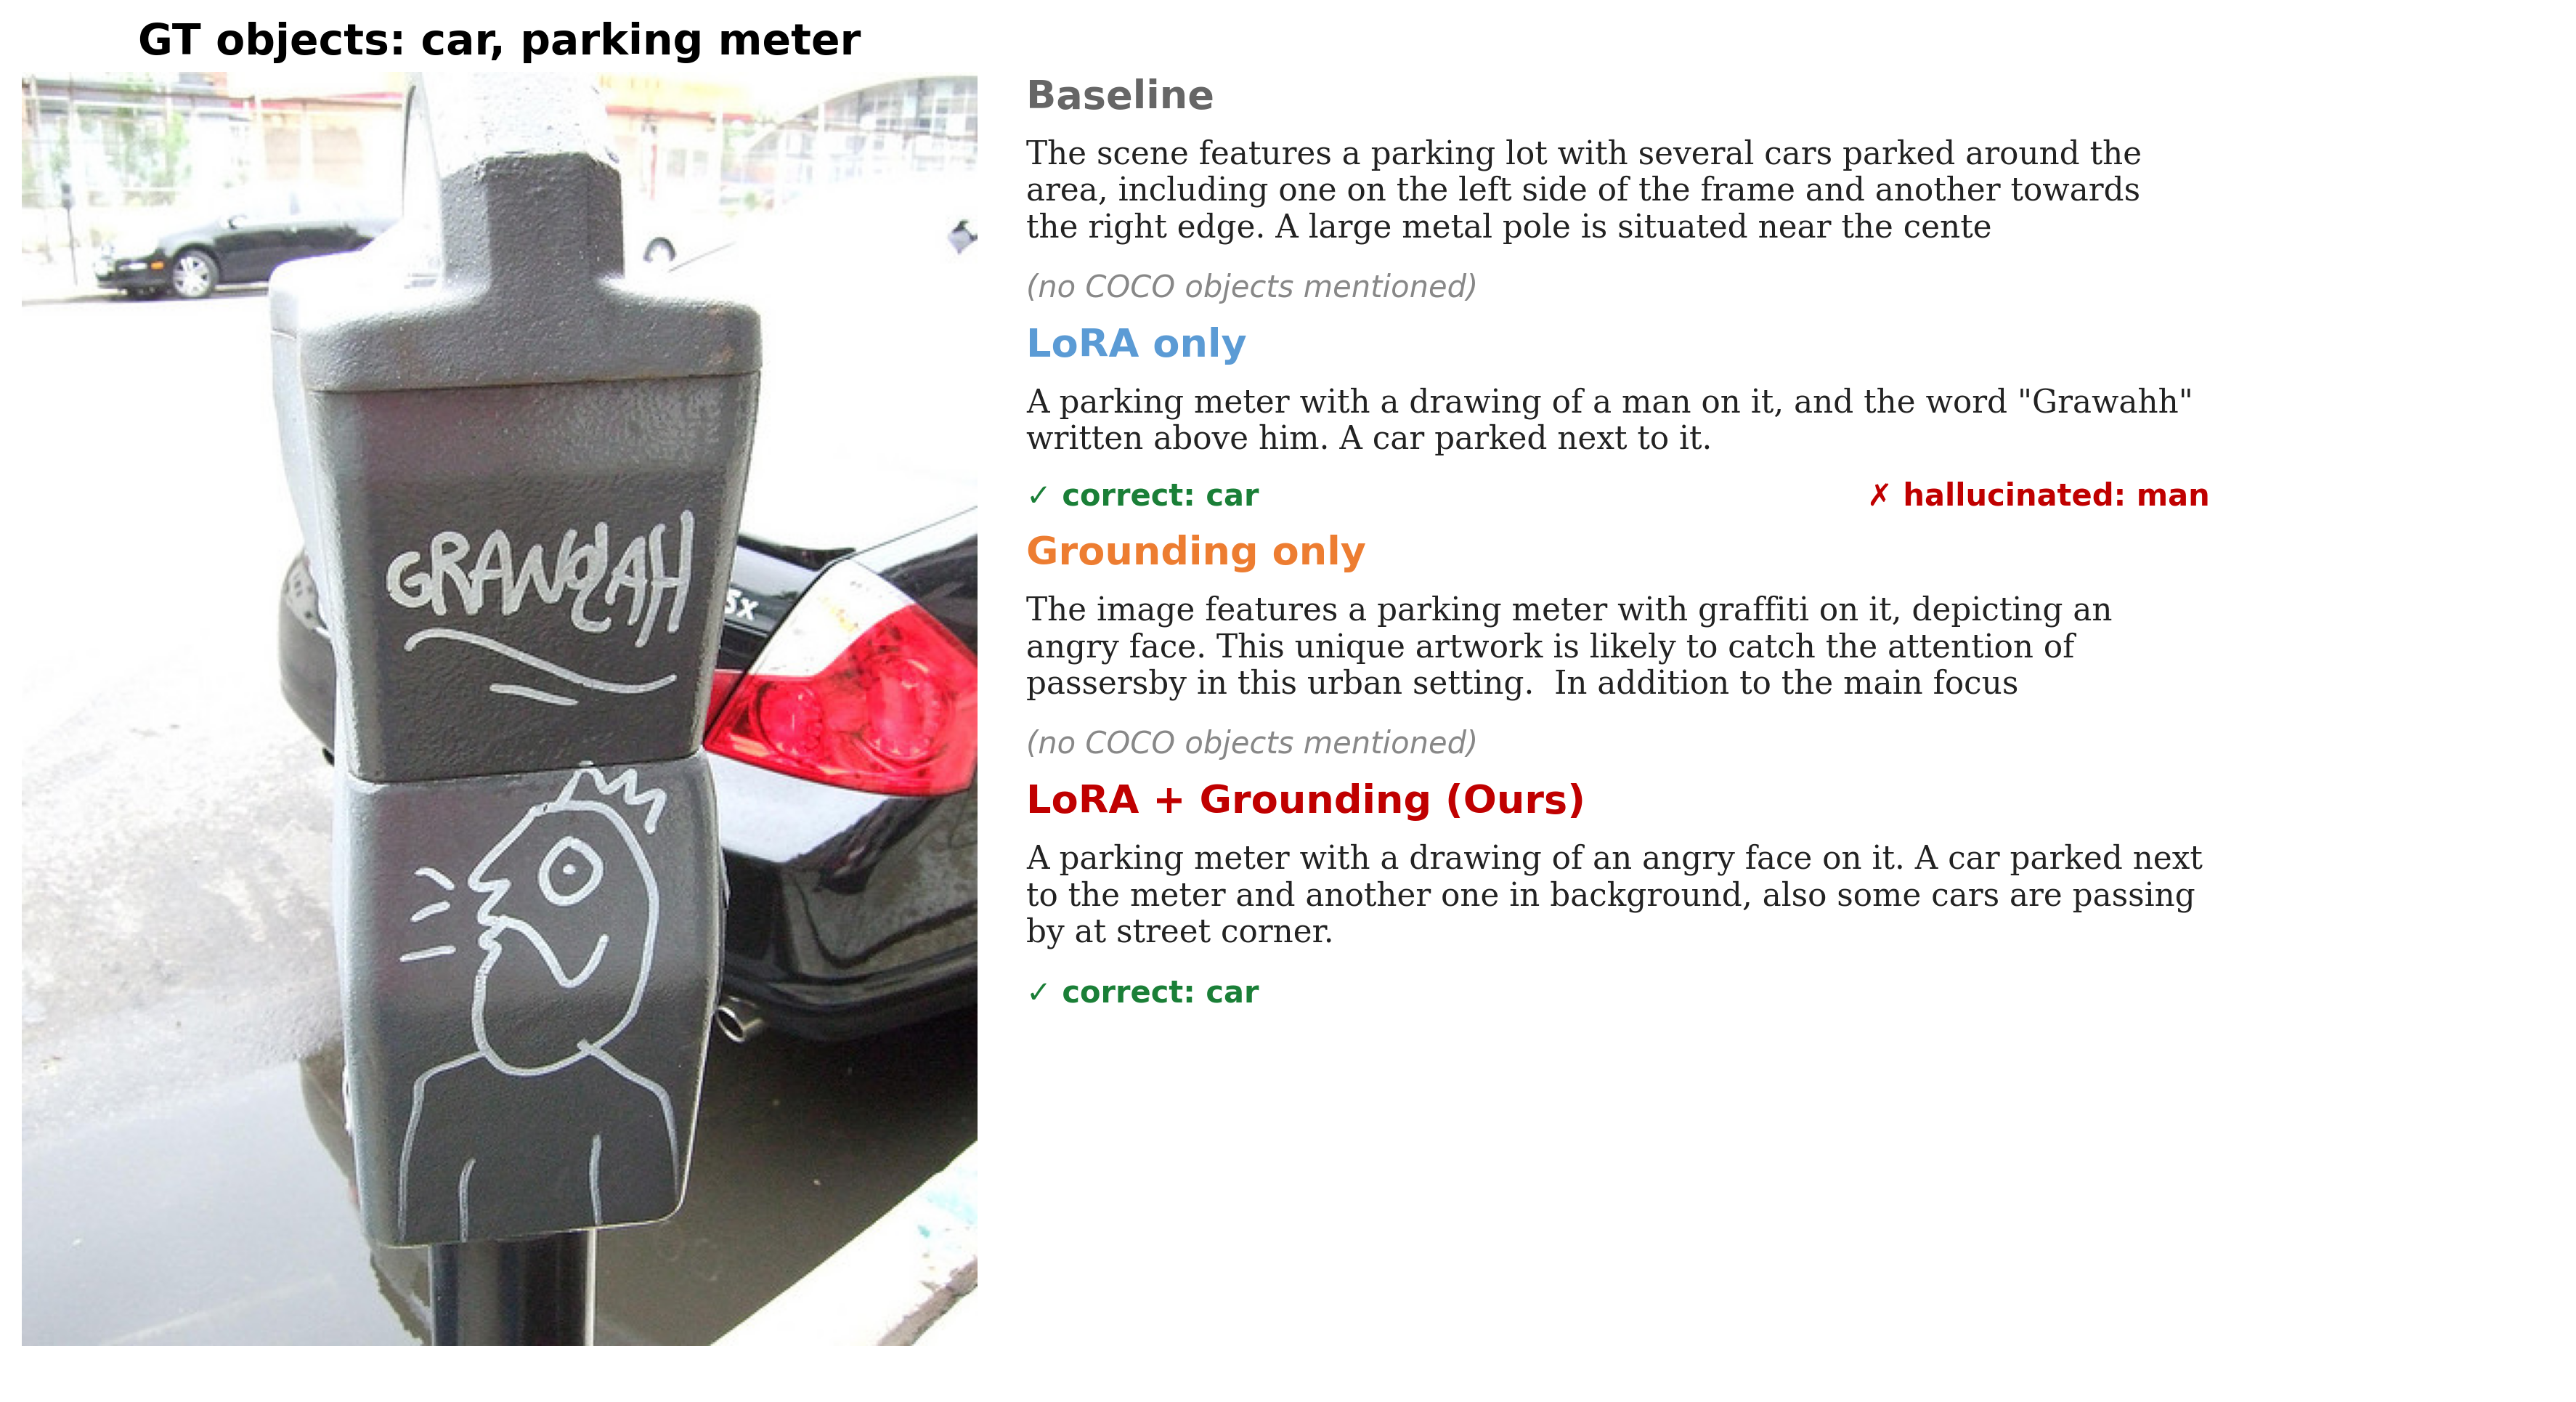
\includegraphics[width=0.97\textwidth]{diagram4_qualitative_example.png}
  \caption{Qualitative example from the poster. The full method keeps the correct object mention while avoiding the extra hallucinated object produced by the LoRA-only variant.}
  \label{fig:qualitative}
\end{figure*}

\section{Discussion}
The main claim of the project is not that hallucination can be eliminated through a small patch, but that a meaningful part of the behavior is localized enough to be manipulated surgically. Updating 32 heads out of 1024 is sufficient to change caption behavior in a measurable way. This is the strongest evidence we found in favor of the original proposal hypothesis.

The results also show why hallucination mitigation should not be evaluated through a single metric. Lower CHAIR does not automatically imply better captions. In our final system, the largest hallucination gains come with shorter outputs and a modest drop in ground-truth object recall. A useful captioning model must remain grounded, informative, and fluent at the same time; suppressing one failure mode too aggressively can introduce another.

Finally, the two intervention points serve different roles. LoRA performs most of the correction, while the grounding controller acts as a residual safety mechanism that catches some remaining weakly grounded steps. That complementarity is the clearest system-level lesson from the project.

\section{Limitations and future work}
There are several limitations to the current study. First, CHAIR depends on COCO object annotations and a hand-built synonym list, so it remains a proxy for visual truth rather than a complete evaluation of factual grounding. Second, the grounding controller uses attention as a heuristic signal rather than a full causal test at inference time. Third, our final metrics show a real tradeoff between hallucination suppression and caption richness. Finally, some smaller notebook runs produced visibly degraded or repetitive text, suggesting that the Stage 2 objective could be better tuned.

Several next steps follow naturally. A better version of Stage 2 could include an explicit fluency-aware or length-aware regularizer. The controller could also move beyond a fixed object vocabulary toward a softer semantic penalty. More broadly, it would be useful to test whether the same small-head intervention strategy transfers to other vision-language backbones and to complement CHAIR with human evaluation of usefulness and readability.

\section{Conclusion}
This project asked whether hallucination in LLaVA-1.5-7B could be reduced through causally targeted intervention on a small subset of attention heads. Our final answer is yes, but with an important qualification. By identifying hallucination-linked heads, applying LoRA only to those heads, and adding inference-time attention grounding, we obtain a substantial reduction in hallucination while changing only about 3.1\% of the model's attention heads.

At the same time, the final system becomes more conservative: captions are shorter, and ground-truth object recall decreases slightly. The overall picture is therefore balanced. Causally targeted adaptation appears to be a promising direction for hallucination mitigation, especially when paired with a simple decoding safeguard, but future work should focus on preserving fluency and coverage while retaining the gains in grounding.

\bibliographystyle{abbrv}
\bibliography{references}

\end{document}
